\documentclass[UTF8]{ctexart}
\usepackage[a4paper,text={150true mm,224true mm},top=35.5true mm,left=30true mm,head=5true mm,headsep=2.5true mm,foot=8.5true mm]{geometry}

\usepackage{titlesec}
\usepackage{amsmath}
\CTEXsetup[format={\large\bfseries}]{section}  

\title{Unsupervised Domain Adaptation by Backpropagation\\基于反向传播的无监督域自调整}
\author{Yaroslav Ganin\\Victor Lempitsky\\ 【译】 jinxiu.qi}
\begin{document}
\maketitle
\begin{abstract}
高性能的深度结构往往训练于一个大规模的数据集中,而在某些特定的任务中,当缺失样本标签时,假设我们拥有一些性质相同但域不相同的标签数据(比如合成图像),那么一种富于吸引力的选择是域自调整方法(domain adaptation)。本文中,我们将提出一种深度结构下新的域自调整方法,它可以在大量拥有标签的源域( source domain)样本和大量没有标签的目标域(target domain)样本中训练(在目标域中的样本,标签不是必须的)。

在训练阶段,我们的方法将促使“深层”特征的产生,所谓“深层”特征,即1)在源域中的学习任务中表现出判别性2)在域之间具备移位不变性。我们将会看到,这种自适行为可以在几乎所有的前-后向模型中实现,只需要在原有的基础上添加少量的标准层以及一个新的“逆梯度(gradient  reversal)”层,扩展后的结构依然可以使用标准的反向传播算法进行训练。

总的说来,这个方法基于现有的深度学习计算框架做一点轻微的开发便可实现,在一系列的图像识别任务中表现十分出色,在域存在大移位的数据集中实现良好的自适性,并且打破了之前领先者的记录。
\end{abstract}

\section{导言}
自己去看论文,不翻了。
\section{相关工作}
自己去看论文,不翻了。
\section{深度域自调整}
\subsection{模型}
现在我们详细得讨论深度域自调整模型细节。首先,我们假设模型的输入样本$x \in X$,其中$X$为输入空间。事实标签(输出)$y$来自标签空间$Y$,我们还假设分类问题中$Y$的状态是有限集合($Y = \{1, 2, \cdots, L\}$),但实际上我们的方法是通用的,可以应用于任何一个其他深度前馈模型所能处理的标签空间。接着,我们假设存在两个$X\otimes Y$下的分布$\mathcal{S}(x, y)$和$\mathcal{T}(x, y)$,分别代表源分布和目标分布(或者源域和目标域),这两个分布都假定是复杂且未知的,此外,两者是相似而不相同的(换言之,通过某些“域移位”可以将$\mathcal{S}$移动到$\mathcal{T}$)。


我们的最终目标是能对一个出自于目标分布的样本$x$预测其标签$y$。在训练时,通过边缘分布$\mathcal{S}(x)$和$\mathcal{T}(x)$,我们可以获取源域和目标域分布中的大量样本集$\{x_1, x_2, \cdots, x_N\}$。第$i$个样本的域标签,我们用二元变量$d_i$标识,它指明样本$x_i$是出自于源分布($x_i \sim \mathcal{S}(x)$,此时$d_i=0$)还是目标分布($x_i \sim \mathcal{T}(x)$,此时$d_i=1$)。对于出自于源分布的样本(即$d_i=0$),其对应的标签$y_i \in Y$在训练时是已知的,而对于出自于目标分布的样本,在训练时它们的标签是未知的,在测试时我们需要做的是预测源自目标分布的样本。

现在我们定义一个深度前馈模型用于将输入$x$映射为它的标签$y$和域标签$d \in \{0, 1\}$,我们将这种映射分解为三个部分。我们假设输入$x$首先通过一个特征提取器$G_f$映射为一个$D$维特征$f \in R^D$,这个特征映射过程可能包含很多层前馈结构,里面所有的参数我们用一个统一的标识$\theta_f$表示,即:$f = G_f(x;\theta_f)$。随后,特征向量$f$通过标签预测器$G_y$映射到预测输出$y$,这个过程中的参数我们记为$\theta_y$。最后,对于同一个特征向量$f$,通过域分类器$G_d$映射为域标签$d$,其参数记为$\theta_d$,整个结构如图\ref{img: model architecture}所示。
\begin{figure}[htbp]
\begin{center}
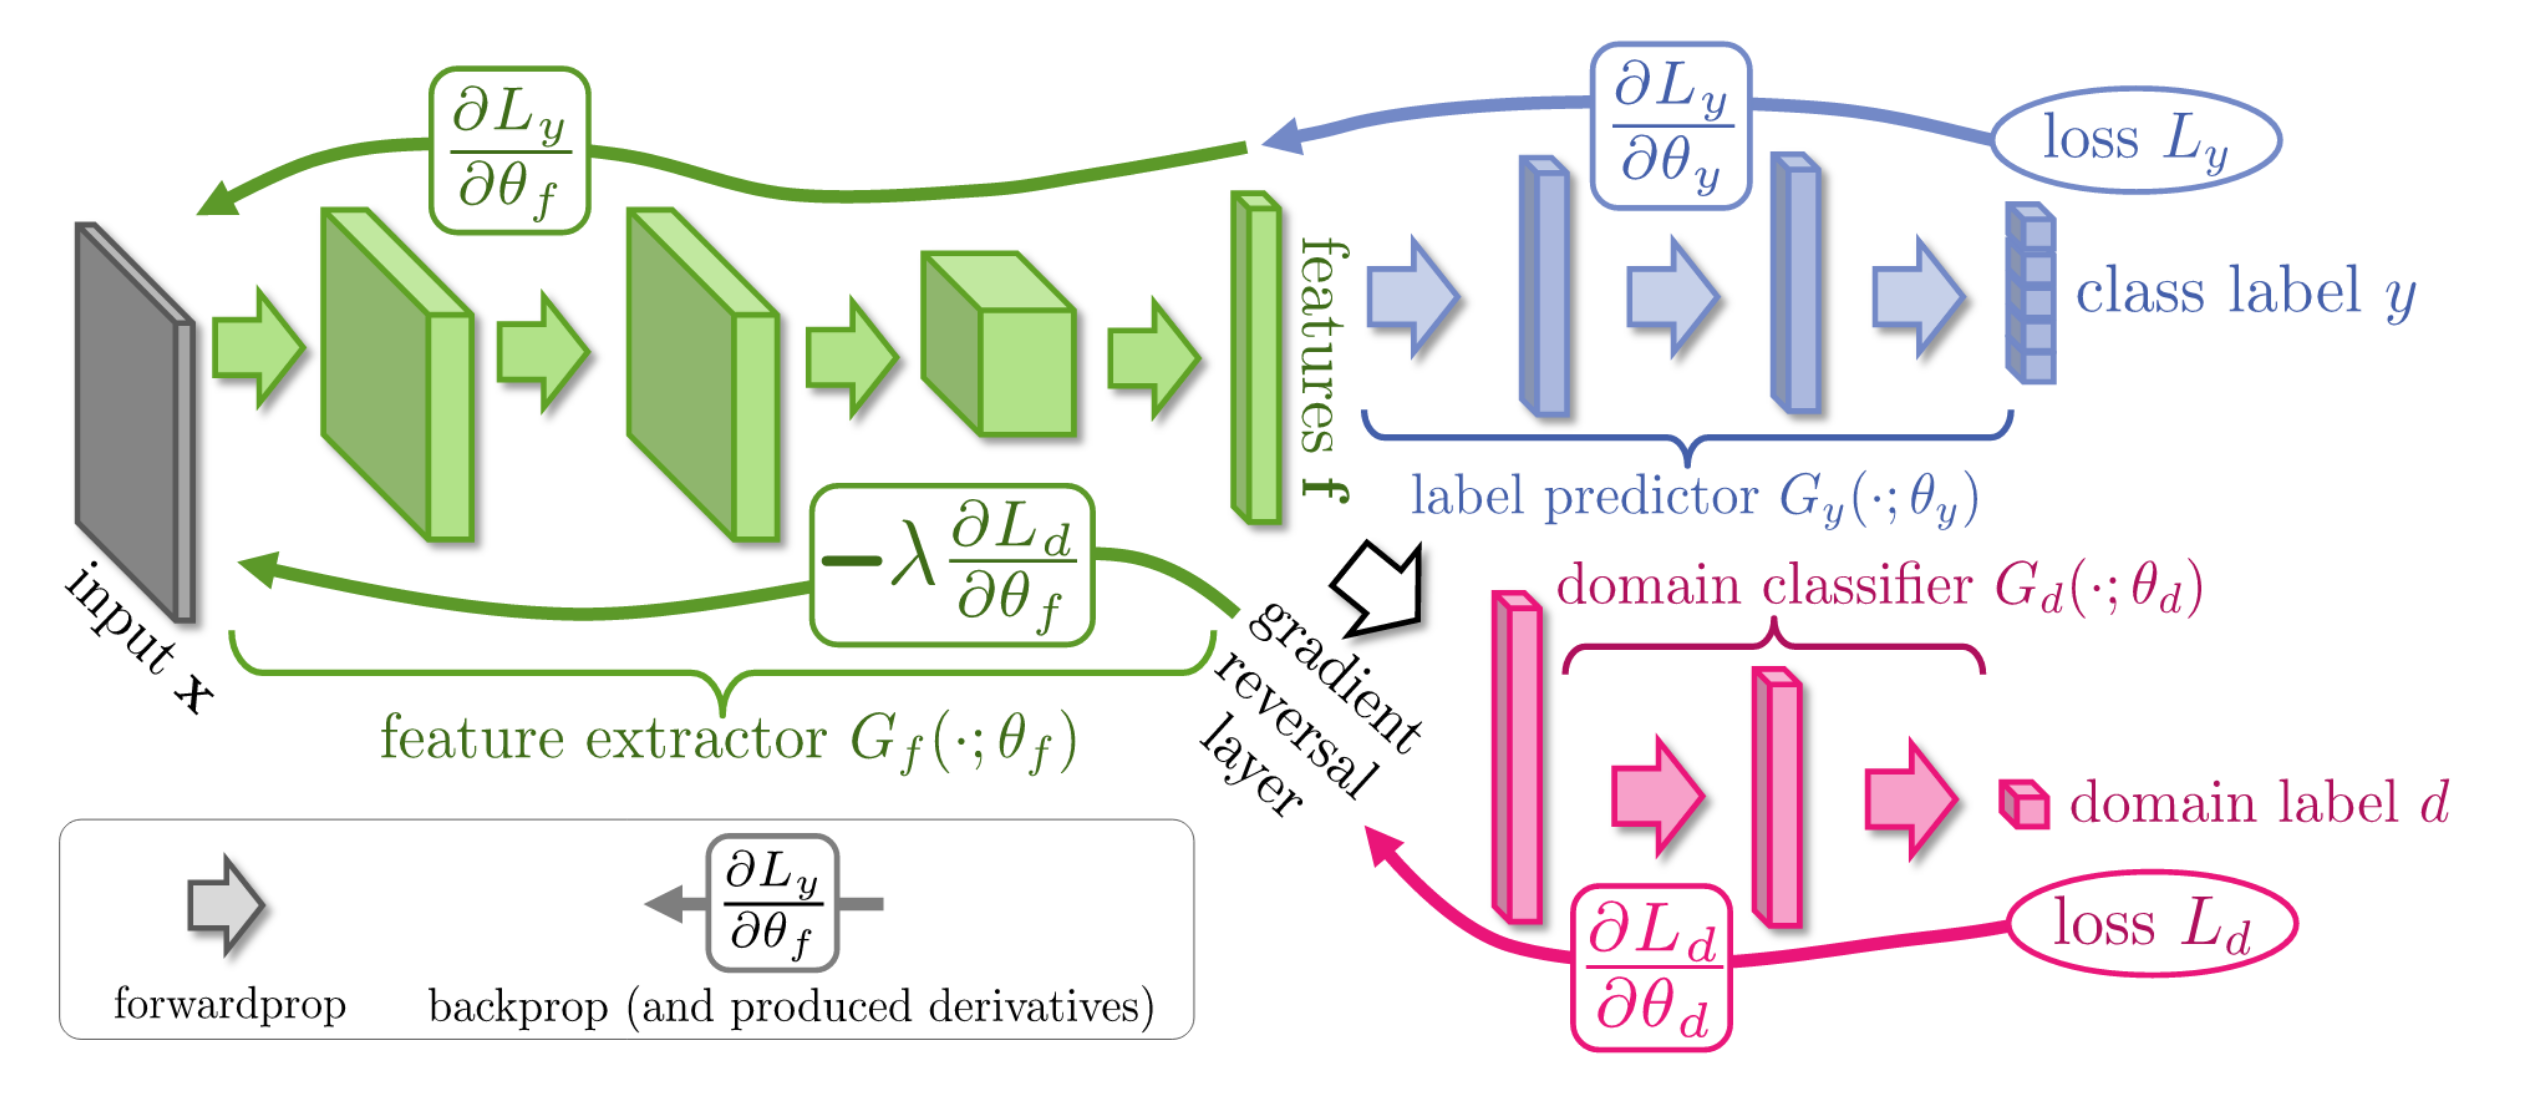
\includegraphics[width=0.9\linewidth]{image/model_architecture.png}
\end{center}
\caption{该模型结构包含了一个深度的特征提取器(绿色)和一个深度的标签预测器(蓝色),这两块与传统的前馈结构没什么区别。无监督的域自调整模型的差异在于它在特征提取器的后面通过一个逆梯度层增加了域分类器(红色),逆梯度层在反向传播训练过程中将梯度乘上一个特定的负常数,确保两个域中的特征分布式相似的,即通过特征无法区分样本源自于哪个域。与标准结构对比,其他方面没有太大差异,在训练过程中最小化预测标签的损失函数(只针对源域样本)的同时,最小化域分类的损失函数(针对所有的样本)。}
\label{img: model architecture}
\end{figure}

在学习阶段,我们的目标是在训练集中有标签的部分(即源域)中最小化标签预测的损失函数,因此特征提取器和标签预测器的优化目标是最小化源域样本的经验损失,确保特征$f$具备判别性并且在源域上通过特征提取器和标签预测器两者结合能获得一个较好的分类性能。

与此同时,我们希望特征$f$具备移位不变性,换言之,我们希望分布$S(f) = \{G_f(x;\theta_f)|x\sim S(x)\}$与分布$T(f) = \{G_f(x;\theta_f)|x\sim T(x)\}$是相似的,在方差偏移(covariate shift)的假设下,我们便可以在目标域中获得于源域相同的准确率。测量分布$S(f)$和$T(f)$的不相似度并不容易,假设$f$是高维的,在训练过程中,分布自身又经常会发生变化,假定我们通过某些方式,训练得到域分类器的参数$\theta_d$用于描述两个特征分布,那么一种估计不相似度的方法是观察域分类器$G_d$的损失。

我们的灵感源自于此,在训练阶段,为了获取具备域不变性的特征,我们寻求特征映射的参数$\theta_f$使得域分类的损失最大化(从而使得两个特征空间尽可能的相似),同时,寻求域分类器的参数$\theta_d$最小化域分类的损失,此外,我们还需要最小化标签预测器的损失。

正式地,我们考虑下面这个方程
\begin{equation}
\begin{split}
E(\theta_f, \theta_y, \theta_d)  &= \sum\limits_{\substack{i=1, \cdots, N\\  d_i=0}}L_y(G_y(G_f(x_i;\theta_f);\theta_y),yi) 
- \lambda\sum\limits_{i=1, \cdot, N}L_d(G_d(G_f(x_i; \theta_f); \theta_d), yi)     \\
&= \sum\limits_{\substack{i=1, \cdots, N\\  d_i=0}}L_y^i(\theta_f, \theta_y) - \lambda\sum\limits_{i=1, \cdots, N}L_d^i(\theta_f, \theta_d)
\end{split}
\label{equ: expect}
\end{equation}
式中,$L_y(\cdot, \cdot)$是标签预测器的损失函数(比如多项式),$L_d(\cdot, \cdot)$是域分类器的损失(比如对数似然),$L_y^i$和$L_d^i$表示第$i$个训练样本对应的损失值。

基于我们的思路,我们的目标是在泛函中寻求一组参数$\hat{\theta}_f, \hat{\theta}_y, \hat{\theta}_d$是的它落入鞍点
\begin{equation}
(\hat{\theta}_f, \hat{\theta}_y) = \arg \min\limits_{\theta_f, \theta_y}E(\theta_f, \theta_y, \hat{\theta}_d)
\label{equ:saddle point f and y}
\end{equation}
\begin{equation}
\hat{\theta}_d = \arg \max\limits_{\theta_d}E(\hat{\theta_f}, \hat{\theta_y}, \theta)
\label{equ:saddle point d}
\end{equation}

在鞍点中,域分类器的参数$\theta_d$最小化域分类损失(因为式\eqref{equ: expect}中它的符号是负号),而标签预测器最小化标签预测损失。特征映射的参数$\theta_f$最小化标签预测的损失,但是最大化域分类的损失(为了域不变性),参数$\lambda$控制训练过程中这两个目标的权重。

接下来,我们证明标准的梯度下降方法可以用来寻求鞍点\eqref{equ:saddle point f and y}-\eqref{equ:saddle point d}。


\subsection{使用反向传播进行最优化}
鞍点\eqref{equ:saddle point f and y}-\eqref{equ:saddle point d}可以通过下面的随机更新策略获取:
\begin{equation}
\theta_f ~~~~\leftarrow~~~~ \theta_f - \mu(\frac{\partial L_y^i}{\partial \theta_f} - \lambda\frac{\partial L_d^i}{\partial \theta_f} )
\label{equ: update rule 1}
\end{equation}
\begin{equation}
\theta_y ~~~~\leftarrow~~~~ \theta_y - \mu\frac{\partial L_y^i}{\partial \theta_y}
\label{equ: update rule 2}
\end{equation}
\begin{equation}
\theta_d ~~~~\leftarrow~~~~ \theta_d - \mu\frac{\partial L_d^i}{\partial \theta_d}
\label{equ: update rule 3}
\end{equation}
其中$\mu$为学习率(可以随时间变化)。

式\eqref{equ: update rule 1} - \eqref{equ: update rule 3}与传统的前馈深度结构中使用的SGD十分类似,你可以想象为一种将特征提取器与标签预测器和域分类器结合的前馈结构,不同的地方在于\eqref{equ: update rule 1}中多了一个因子$-\lambda$(这点差异非常重要,如果没有这个因子,为了最小化域分类损失,SGD将使得域间的特征不相似)

尽管没有办法直接通过SGD实现式\eqref{equ: update rule 1}-\eqref{equ: update rule 3},但我们仍然有必要将其归纳到SGD上,因为SGD(以及它的变体)是很多深度学习计算框架的基础算法。

幸运的是,这种归纳可以引入一种特殊的逆梯度层(gradient reversal layer, GRL)来解决。逆梯度层没有对应的参数(不考虑元参数$\lambda$,因为它在反向传播中不更新),在前向传播过程中,GRL进行等价映射,而在反向传播中,GRL接收它后面层传播回来的梯度,然后乘上参数$-\lambda$,接着将它继续传到前面的层中去。通过现有的面向对象的深度学习框架很容易实现这种层结构,只需要重写前馈的处理逻辑(等价映射)、反馈逻辑(乘上一个常数)以及更新策略(由于没有参数,所以不需要做任何处理)。

上面提到的GRL会被插入到特征提取器和域分类器中间,正如图\ref{img: model architecture}所示。当反向传播处理过程进展到GRL层时,损失函数的偏导数是GRL的下游(即$L_d$)相对于GRL的上游的层参数(即$\theta_f$)的偏导再乘上$-\lambda$,也就是说$\frac{\partial L_d}{\partial \theta_f}$被替换为$-\lambda\frac{\partial L_d}{\partial \theta_f}$。因此,使用SGD来更新\eqref{equ: update rule 1}-\eqref{equ: update rule 3}可以是的式\ref{equ: expect}收敛到鞍点。

从数学的角度上而言,我们可以将逆梯度层视为一个通过下面两个(互斥的)描述前/反馈行为的等式定义出的“伪函数”$R_\lambda(x)$:
\begin{equation}
R_\lambda(x) = x
\end{equation}
\begin{equation}
\frac{dR_\lambda}{dx} = -\lambda I
\end{equation}
其中$I$为单位矩阵。随后我们便可以定义关于$(\theta_f, \theta_y, \theta_d)$的“伪函数”作为我们SGD的优化目标:
\begin{equation}
\begin{split}
\widetilde{E}(\theta_f, \theta_y, \theta_d) =& \sum\limits_{\substack{i=1, \cdots, N\\  d_i=0}}L_y(G_y(G_f(x_i;\theta_f);\theta_y),yi) \\
&+\sum\limits_{i=1, \cdot, N}L_d(G_d(R_\lambda(G_f(x_i; \theta_f)); \theta_d), yi)
\end{split}
\label{equ: wide tilde expect}
\end{equation}

通过更新策略\eqref{equ: update rule 1}-\eqref{equ: update rule 3},SGD可以优化式\eqref{equ: wide tilde expect}从而获取同时具备域不变性和判别性的特征。学习完毕后,标签预测器$y(x) = G_y(G_f(x_i;\theta_f);\theta_y)$可以用来预测来自于目标域中的样本(正如源域中的一样的操作)。



\subsection{与$\mathcal{H}\Delta\mathcal{H}$的关系}
本小节中,我们给出一个我们的方法在$\mathcal{H}\Delta\mathcal{H}$-距离上的简要分析,这种距离常用于非保守域自调整理论。一般地
\begin{equation}
d_{\mathcal{H}\Delta\mathcal{H}}(\mathcal{S}, \mathcal{T}) = 2 \sup\limits_{h1, h2 \in \mathcal{H}} | P_{f\sim \mathcal{S}}[h_1(f) \neq h_2(f)] - P_{f\sim \mathcal{T}}[h_1(f) \neq h_2(f)]|
\end{equation}
定义了假设空间$\mathcal{H}$下两个分布$\mathcal{S}$和$\mathcal{T}$的差异距离(discrepancy distance),通过这个标识,给定某个分类器$h$在源域的性能$\varepsilon_\mathcal{S}(h)$时,我们可以获取它在目标域分布$\mathcal{T}$下性能$\varepsilon_\mathcal{T}(h)$的概率上界:
\begin{equation}
\varepsilon_\mathcal{T}(h) \leq \varepsilon_\mathcal{S}(h) + \frac{1}{2}d_{\mathcal{H}\Delta\mathcal{H}}(\mathcal{S}, \mathcal{T}) + C
\end{equation}
其中$\mathcal{S}$和$\mathcal{T}$是源域和目标域对应的分布,而$C$不依赖于特定的$h$。

现在考虑由特征提取器$G_f$和一族标签预测器$\mathcal{H}_p$生成的表示空间下特定的$\mathcal{S}$和$\mathcal{T}$,我们假设域分类器的族$\mathcal{H}_d$足够丰富以至于它包含$\mathcal{H}_p$假设集的对称差集\footnote{即由A 中或B 中的元素 但不同时属于A 和B 的元素形成的集合}:
\begin{equation}
\mathcal{H}_p\Delta\mathcal{H}_p = {h|h=h_1\oplus h_1, h_1, h_2 \in \mathcal{H}_p}
\end{equation}

这并不是一个不切实际的假设,因为我们可以随意地选取任何一个我们想要地$\mathcal{H}_d$,例如,我们可以将域分类器设置为两个标签预测器的副本的级联(层-层结构),用非线性感知器去学习异或函数。假定我们的假设成立,那么很显然训练$G_d$跟估计$d_{\mathcal{H}_p\Delta\mathcal{H}_p}(\mathcal{S}, \mathcal{T}) $是高度相关的工作,确实也是这样的:
\begin{equation}
\begin{split}
d_{\mathcal{H}_p\Delta\mathcal{H}_p}(\mathcal{S}, \mathcal{T}) &= 
2 \sup\limits_{h\in \mathcal{H}_p\Delta\mathcal{H}_p} | P_{f\sim \mathcal{S}}[h(f) = 1] - P_{f\sim \mathcal{T}}[h(f) = 1] | \\
& \leq 2 \sup\limits_{h\in \mathcal{H}_d} | P_{f\sim \mathcal{S}}[h(f) = 1] - P_{f\sim \mathcal{T}}[h(f) = 1] | \\
& = 2 \sup\limits_{h\in \mathcal{H}_d} | 1 - \alpha(h) |  \\
& =  2 \sup\limits_{h\in \mathcal{H}_d} | \alpha(h) - 1| 
\end{split}
\end{equation}
其中,$\alpha(h) = P_{f\sim\mathcal{S}}[h(f) = 0] + P_{f\sim\mathcal{T}}[h(f) = 1]$是最优化$G_d$取得的最大值。

因此,最优的分类器使得$d_{\mathcal{H}_p\Delta\mathcal{H}_p}(\mathcal{S}, \mathcal{T})$取得上界。同时,逆梯度的反向传播改变了表达空间,$\alpha(G_d)$变得更小,从而降低了$d_{\mathcal{H}_p\Delta\mathcal{H}_p}(\mathcal{S}, \mathcal{T})$,以至于$\varepsilon_\mathcal{T}(G_y)$更逼近于$\varepsilon_\mathcal{S}(G_y)$。


\section{实验}
自己去看论文,不翻了。

\subsection{结果}
自己去看论文,不翻了。
\section{讨论}
自己去看论文,不翻了。

\end{document}